\documentclass[10pt, a4paper]{article}
\usepackage{a4wide}

\usepackage[ngerman]{babel}
\usepackage[utf8]{inputenc}
\usepackage[T1]{fontenc}

\usepackage{parskip}
\usepackage{graphicx}
%\usepackage{amsmath}

\newcommand{\ra}{$\rightarrow$ }
\newcommand{\Ra}{$\Rightarrow$ }
\newcommand{\la}{$\leftarrow$ }
\newcommand{\La}{$\Leftarrow$ }

\newcommand{\angstrom}{\mbox{\normalfont\AA}}

\newcommand{\delt}{\mathrm{d}}

\newcommand{\subsubsubsection}[1]{\paragraph{#1}\mbox{}\\}

\setcounter{section}{-1}

% show paragraphs in the TOC
\setcounter{tocdepth}{4}
\setcounter{secnumdepth}{4}

\title{Werkstofftechnik WS 16/17}


\begin{document}

\maketitle
\tableofcontents

\let\thefootnote\relax\footnotetext{Anmerkungen:}
\let\thefootnote\relax\footnotetext{- Fehlerfunde bitte an s75662@htw-dresden.de schicken, danke :)}
\let\thefootnote\relax\footnotetext{- Vorhandene handschriftliche Grafiken sind Platzhalter und werden in naher Zukunft noch digitalisiert.}

\newpage

\section{Organisatorisches}

Prof. Gorbunoff

Literaturempfehlung: Werkstoffe der Elektrotechnik Ivers-Tiffeé von Münch Teubner

Zur Prüfung ist alles ausschließlich handschriftliche zugelassen.

\section{Werkstoffeigenschaften}

\begin{tabular}{c c c c}
	Eigenschaft & Stimulus & typische Reaktion & Kenngröße \\
	\hline
	mechanische & mechanische Kraft & Verformung, Bruch & $E$, $\sigma$ \\
	thermische & Energiezufuhr & Temperaturanstieg & $C_v$, $\lambda$ \\
	elektrische & E-Feld & Strom, Polarisation & $p$, $\epsilon$ \\
	optische & Licht & Farbe, Brechung & $R$, $T$, $n$ \\
	magnetische & H-Feld & magnetische Anziehung & $\mu$, $H_c$\\
\end{tabular}

Werkstoffe mit mechanischen Eigenschaften sind Konstruktionswerkstoffe. Die anderen sind Funktionswerkstoffe.

\subsection{Aufbau der Atome und Periodensystem der Elemente}

\subsubsection{Bohr'sches Atommodell und Wasserstoffatom}

\begin{minipage}{.3\textwidth}
	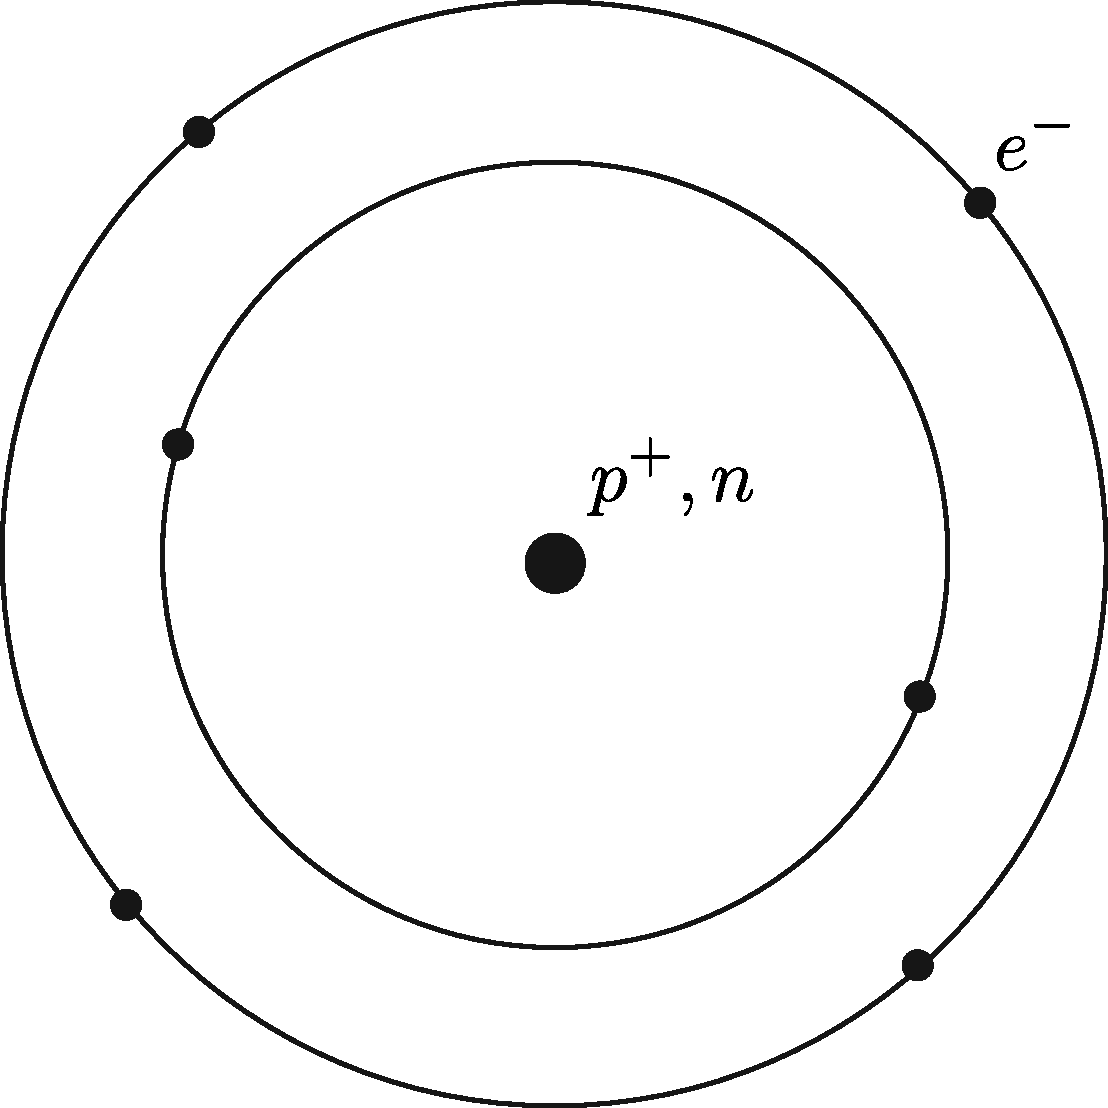
\includegraphics[width=\textwidth]{img/1_1}
\end{minipage}\hfill
\begin{minipage}{.65\textwidth}
	\begin{itemize}
		\item Kern: ca. $10^{-5}...10^{-4} \angstrom$ ($1\angstrom = 10^{-10}m$)
		\begin{itemize}
			\item Neutronen ($n$): $q_n = 0$
			\item Protonen ($p^+$): $q_p = e = 1{,}60 \cdot 10^{-19}C$
		\end{itemize}
		\item Elektronenhülle: R ca. $0{,}5...2{,}5\angstrom$
		\begin{itemize}
			\item Elektronen ($e^-$): $q_e = -e = -1{,}60 \cdot 10^{-19}C$ \\ 
			$m_e << m_n$ \Ra Die ganze Masse des Atoms ist nahezu im Kern konzentriert.
		\end{itemize}
		\item Orbital: Aufenthaltsraum des Elektrons im Raum
	\end{itemize}
\end{minipage}

\underbar{Energieniveaus von Elektronen in Atomen}

Wenn Elektronen von einem Orbital zu einem anderen springen, entstehen Protonen oder werden absorbiert. \ra Diese Übergänge sind also reversibel.

Atome haben diskrete Energieniveaus (Orbitale). Atome müssen nicht neutral sein.

Diskrete Energieniveaus: Bindungsenergien von Elektronen im Atom

Valenzelektronen (ganz außen) haben die geringsten Bindungsenergien.

\subsubsection{Quantenmechanik und die Elektronenhülle}

<Buch 1.3>

Alle Elektronen mit der selben Hauptquantenzahl ($n$) bilden eine Elektronenschale (K-Schale ist die innerste).

Die Bahndrehimpulsquantenzahl ($l$) bestimmt die Form.
\begin{itemize}
	\item liegt zwischen 0 und $n-1$
	\item alle Elektronen mit der selben Nebenquantenzahl (Bahndrehimpuls-QZ) bilden eine Unterschale.
\end{itemize}

Orientierungsquantenzahl ($m_l$)
\begin{itemize}
	\item bestimmt räumliche Orientierung
	\item betrifft nur nicht-kugelförmige Orbitale
	\item ganzzahlig, positiv oder negativ, zwischen 0 und $\pm l$
\end{itemize}

\underbar{Besetzung der Elektronenzustände}
\begin{itemize}
	\item Prinzip der Energieminimierung\\
		Ein Elektron besetzt bei mehreren Möglichkeiten das Orbital mit der niedrigsten Energie, d.h. meist das innerste
	\item Pauli-Ausschließungsprinzip \\
		In einem Atom dürfen keine zwei \underbar{identischen} Elektronen einen und denselben Quantenzustand besitzen. Elektronen unterscheiden sich in erster Linie im Spin.
\end{itemize}

Eigendrehimpulsquantenzahl ($m_s$) ``\textit{Spin}''
\begin{itemize}
	\item positiv oder negativ $\frac{1}{2}$ (``spin up'', ``spin down'')
\end{itemize}
\Ra mit zwei Elektronen mit unterschiedlichem Spin ist die K-Schale voll besetzt, da sie nur eine Unterschale hat.

<Buch 1.4>

<Buch 1.9>

Nach 3p kommt 4s, da 4s ein tieferes Niveau hat als 3d.

\subsubsection{Das Periodensystem der Elemente}

Das Periodensystem spiegelt die Besetzungsreihenfolge der Elektronen.

\subsection{Die Aggregatszustände der Materie}

\underbar{Aggregatszustände:} qualitativ unterschiedliche, temperatur- und druckabhängige Erscheinungsformen der Stoffe

\begin{itemize}
	\item Edelgase: keine reguläre Atomordnung
	\item Molekulare Gase: Nahordnung\\
		Moleküle sind regelmäßig und innerlich identisch aufgebaut
	\item Flüssigkeiten: Nahordnung\\
		Ordnung besteht auch hier nur auf Molekularebene
	\item Kristalle: Fernordnung\\
		Ordnung, die sich deutlich weiter als über einen Baustein erstreckt
\end{itemize}

\subsubsection{Gase und Flüssigkeiten}

\begin{center}
	\includegraphics[width=.8\textwidth]{img/2_1_int}
\end{center}

\underbar{Festkörper:}
\begin{itemize}
	\item praktisch inkompressibel
	\item formbeständig
\end{itemize}

\underbar{Flüssigkeit:}
\begin{itemize}
	\item praktisch inkompressibel
	\item leichte Formänderung
	\item haben keine bestimmte Gestalt
	\item haben freie Oberfläche
	\item nimmt die Form des Behälters an, in den sie eingegossen wird
\end{itemize}

\underbar{Gas:}
\begin{itemize}
	\item keine bestimmte Gestalt
	\item hochkompressibel
	\item nehmen immer das ganze freie Volumen des Behälters ein
\end{itemize}

\subsubsection{Kristallstrukturen (ideale Kristalle)}

Kristallstruktur: 3d-Anordnung von Atomen, Molekülen oder Ionen in Kristallen

\subsubsubsection{Kristallgitter}

\begin{center}
	\includegraphics[width=.8\textwidth]{img/2_2_int}
\end{center}

\begin{itemize}
	\item \underbar{Kristallgitter:} abstrakte mathematische Darstellung der Kristallstruktur als eine räumlich periodische Anordnung von \underbar{Punkten} (Punktgitter).
	\item Elementarzelle: das Element des Kristallgitters, mit dem durch \underbar{Translationen} das vollständige Kristallgitter \underbar{lückenlos} reproduziert werden kann.
	\item Gitterkonstanten: die Beträge der Kanten und Winkel der Elementarzelle
	\item Kristallsysteme\\
		\begin{center}
			\includegraphics[width=.8\textwidth]{img/2_3_int}
		\end{center}
		Wichtig für uns: hexagonal, kubisch-primitv, kubisch-raumzentriert und kubisch-flächenzentriert
	\item Bravais Gitter
	\item Atome in der Elementarzelle
		\begin{itemize}
			\item Zahl von Atomen in der Elementarzelle: $N_{EZ}$\\
				$N_{EZ}$ krz: 2; $N_{EZ}$ kfz: 4
			\item Packungsdichte (PD)\\
				$$\frac{\textrm{Atomvolumen in der EZ}}{\textrm{Volumen der EZ}}$$
			\item Koordinationszahl (KZ)\\
				Anzahl nächster Nachbarn jedes Atoms
			\item Miller'sche Indizes
				\begin{itemize}
					\item Ebenen\\
						\begin{center}
							\includegraphics[width=.8\textwidth]{img/2_4_int}
						\end{center}
					\item Richtungen\\
						in kubischen Gittern: $[100] \perp (100)$; $[110] \perp (110)$; $[111] \perp (111)$
						\begin{center}
							\includegraphics[width=.8\textwidth]{img/2_5_int}
						\end{center}
				\end{itemize}
		\end{itemize}
\end{itemize}

\subsubsubsection{Metalle}

\underbar{Kubisch primitives Gitter}

\begin{itemize}
	\item $N_{EZ}$: 1 (cP1)
	\item KZ: 6
	\item PD: 52\%
	\item sehr selten (z.B. Polonium)
\end{itemize}

\begin{minipage}{.4\textwidth}
	\underbar{Kubisch raumzentriertes Gitter}
	\begin{itemize}
		\item $N_{EZ}$: 2 (cI2)
		\item KZ: 8
		\item PD: 68\%
		\item harte Metalle: $\alpha$-Fe, Cr, W, Mo
	\end{itemize}	
\end{minipage}
\begin{minipage}{.6\textwidth}
	\includegraphics[width=\textwidth]{img/2_6_int}
\end{minipage}

\begin{minipage}{.4\textwidth}
	\underbar{Kubisch flächenzentriertes Gitter}
	\begin{itemize}
		\item $N_{EZ}$: 4 (cF4)
		\item KZ: 12
		\item PD: 74\%
		\item weiche Metalle: Au, Ag, Cu, Al, Ni, Pb
	\end{itemize}	
\end{minipage}
\begin{minipage}{.6\textwidth}
	\includegraphics[width=\textwidth]{img/2_7_int}
\end{minipage}

\begin{minipage}{.4\textwidth}
	\underbar{Hexagonal dichteste Packung}
	\begin{itemize}
		\item $N_{EZ}$: 2 (hP2)
		\item KZ: 12
		\item PD: 74\%
		\item Zn, Cd, Hg
	\end{itemize}	
\end{minipage}
\begin{minipage}{.6\textwidth}
	\includegraphics[width=\textwidth]{img/2_8_int}
\end{minipage}

\newpage
\subsubsubsection{Kovalente Kristalle}

\includegraphics[width=\textwidth]{img/2_9_int}

\begin{itemize}
	\item $N_{EZ}$: 8 (cF8)
	\item KZ: 4
	\item PD: 34\%
	\item Diamant, Silizium, Ge
\end{itemize}










\end{document}
